 \providecommand{\main}{../../..}
\documentclass[\main/main.tex]{subfiles}
\begin{document}
\subsection{Esercizio 1}
Dato il seguente problema di PL:

\begin{figure}
  \begin{align*}
    \min z = x_1 + x_2                             \\
    \frac{7}{2}x_1 - 2x_2 + x_3 & = \frac{9}{2}    \\
    3x_1 + x_2 + x_4            & = 3              \\
    \bmx                        & \in \mathbb{N}^4
  \end{align*}
  \caption{Esercizio 1}
\end{figure}

\begin{enumerate}
  \item Si risolva il suo rilassamento continuo.
  \item Se la soluzione ottima non è intera si trovi un opportuno taglio di Gomory in forma frazionaria, lo si aggiunga al tableau e si trovi l'elemento di pivot senza riottimizzare.
  \item Si disegni il vincolo identificato.
\end{enumerate}

\subsection{Soluzione esercizio 1}
\subsubsection*{Rilassamento continuo}
Il valore minimo che la funzione obbiettivo può raggiungere, nel rilassamento continuo, visti i vincoli, è $0$, con $x_1 = 0, x_2 = 0, x_3 = \frac{9}{2}, x_4 = 3$.

\subsubsection*{Verifico ottimalità}
Verifico che la funzione ottenuta sia ottima mediante il metodo degli scarti complementari.

\begin{figure}
  \begin{subfigure}{0.49\textwidth}
    \begin{align*}
      \max z_D = \frac{9}{2}y_1 + 3y_2 \\
      \frac{7}{2}y_1 + 3y_2 & \leq 1   \\
      -2y_1 + 1y_2          & \leq 1   \\
      y_1                   & \leq 0   \\
      y_2                   & \leq 0   \\
      y_1, y_2              & \in \R
    \end{align*}
    \caption{Problema duale}
  \end{subfigure}
  \begin{subfigure}{0.49\textwidth}
    \[
      \begin{cases}
        x_1(\frac{7}{2}y_1 + 3y_2 -1) = 0               \\
        x_2(-2y_1 + 1y_2          -1) = 0               \\
        x_3y_1 = 0                                      \\
        x_4y_2 = 0                                      \\
        y_1(\frac{7}{2}x_1 - 2x_2 + x_3 -\frac{9}{2})=0 \\
        y_2(3x_1 + x_2 + x_4            -3          )=0 \\
      \end{cases}
      \Rightarrow
      \begin{cases}
        y_1 = 0 \\
        y_2 = 0
      \end{cases}
    \]
    \caption{Scarti complementari}
  \end{subfigure}
  \caption{Verifica soluzione ottima}
\end{figure}

La soluzione è confermata ottima $z=z_D=0$.

\subsubsection*{Taglio di Gomory}
La soluzione ottima comprende valori di $x$ non interi, per cui procedo con il taglio di Gomory. Considerando come base $B = \begin{bmatrix}
    x_3, x_4
  \end{bmatrix}$, il problema considerato è già posto in forma canonica:

\begin{figure}
  \begin{table}
    \begin{tabular}{|LLLL|L|}
      \hline
      x_3                   & x_4 & x_1          & x_2 & \tilde{b}    \\
      \hline
      0                     & 0   & 1            & 1   & 0            \\
      \hline
      \rowcolor{green!30} 1 & 0   & \sfrac{7}{2} & -2  & \sfrac{9}{2} \\
      0                     & 1   & 3            & 1   & 3            \\
      \hline
    \end{tabular}
  \end{table}
  \caption{Tableau in forma canonica}
\end{figure}

Costruisco il taglio di Gomory sulla riga evidenziata in verde:

\begin{align*}
  \sum  (a_{ij} - \floor{a_{ij}})x_j \geq b_i-\floor{b_i}                                                                \\
  \rnd{1-\floor{1}}x_3 + 0x_4 + \rnd{\frac{7}{2} - \floor{\frac{7}{2}}}x_1 + 0x_2 \geq \frac{9}{2} - \floor{\frac{9}{2}} \\
  \frac{1}{2}x_1 \geq \frac{1}{2}                                                                                        \\
  x_1 \geq 1
\end{align*}
Aggiungo il nuovo vincolo al tableau:

\begin{figure}
  \begin{table}
    \begin{tabular}{|LLLL|L|}
      \hline
      x_3 & x_4 & x_1          & x_2 & \tilde{b}    \\
      \hline
      0   & 0   & 1            & 1   & 0            \\
      \hline
      1   & 0   & \sfrac{7}{2} & -2  & \sfrac{9}{2} \\
      0   & 1   & 3            & 1   & 3            \\
      0   & 0   & 1            & 0   & 1            \\
      \hline
    \end{tabular}
  \end{table}
  \caption{Tableau in forma canonica}
\end{figure}

A parità di coefficiente di costo ridotto, scelgo la colonna di $x_1$ essendo quella con i coefficienti maggiori. Per l'operazione di pivot posso scegliere sia il termine appena inserito, $1$, sia $3$ poichè il rapporto tra questi ed il rispettivo termine noto risulta uguale.

\subsubsection*{Disegnare il vincolo}
Rappresento il vincolo sul piano $x_1 - x_2$:

\begin{figure}
  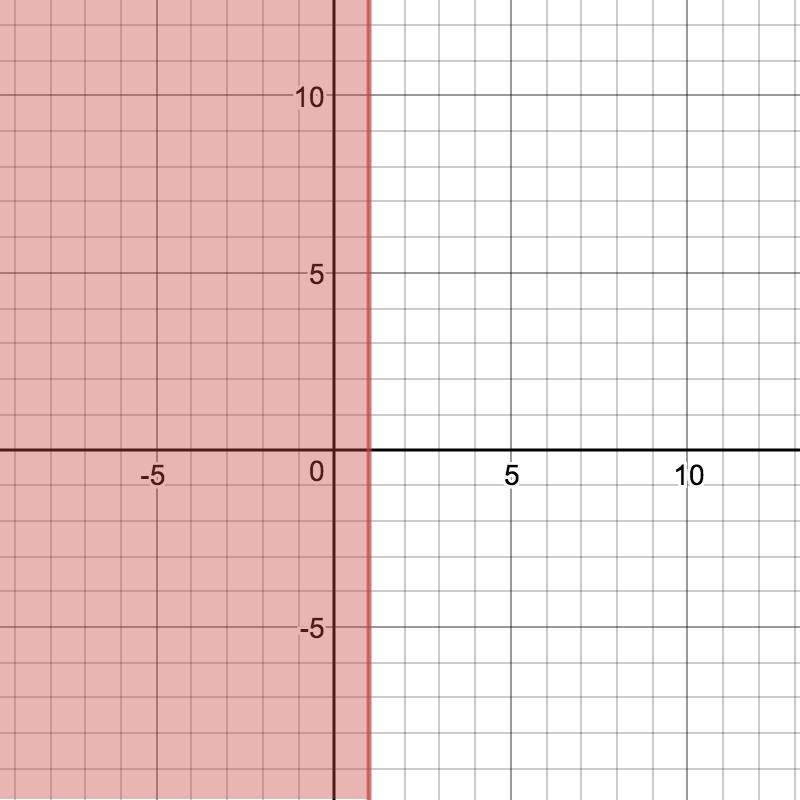
\includegraphics[width=0.4\textwidth]{gomory_2014_09_16}
\end{figure}

\end{document}